% !TEX root = task-3-7-3.tex
% Editable task bank. Append new BankTask blocks at the end of the document.
\documentclass[12pt,a4paper]{article}
\usepackage{physics-textbook}
\usepackage{graphicx,needspace}
\usetikzlibrary{decorations.pathmorphing}
\newif\ifShowSolutions
\ifdefined\TutorEdition
  \ShowSolutionstrue
\else
  \ShowSolutionsfalse % Change to \ShowSolutionstrue to display solutions.
\fi
\newcounter{banktask}
\newsavebox{\BankTaskBox}
\newcommand{\BankTaskContent}[3]{%
  \noindent\textbf{\thebanktask.}\quad #2\par
  \ifShowSolutions
    \Needspace{50mm}% Keep the solution heading with its opening text or diagram.
    #3\par
    \ifdefined\TutorEdition
      \ifcsname TutorSource#1\endcsname
        \nopagebreak\smallskip{\small\csname TutorSource#1\endcsname\par}%
      \fi
    \fi
  \fi
}
\newcommand{\BankTask}[3]{%
  \refstepcounter{banktask}\par\medskip
  \sbox{\BankTaskBox}{\begin{minipage}{\linewidth}%
    \BankTaskContent{#1}{#2}{#3}\end{minipage}}%
  \ifdim\dimexpr\ht\BankTaskBox+\dp\BankTaskBox\relax>\dimexpr\textheight-20mm\relax
    \Needspace{35mm}\BankTaskContent{#1}{#2}{#3}%
  \else
    \Needspace{\dimexpr\ht\BankTaskBox+\dp\BankTaskBox\relax}%
    \noindent\usebox{\BankTaskBox}\par
  \fi
  \medskip
}
\begin{document}
\BookSubsection{3.7.3}{Энергия конденсатора и электрического поля}


% Source sdamgia-11559: https://phys-ege.sdamgia.ru/problem?id=11559
\BankTask{sdamgia-11559}{
Незаряженный конденсатор подключают к батарейке. Как изменились следующие величины в ходе зарядки?\par
$1$. Увеличилась.\par
$2$. Уменьшилась.\par
$3$. Не изменилась.\par
\begin{center}\small\setlength{\tabcolsep}{3pt}\begin{tabular}{|p{0.45\linewidth}|p{0.45\linewidth}|}\hline
Энергия конденсатора & Электрическая емкость
конденсатора\\\hline
 & \\\hline
\end{tabular}\end{center}\par
}{
\smallskip\noindent\textbf{Решение}\par
При подключении батарейки в сети появится напряжение, поэтому энергия конденсатора увеличится, а его электрическая емкость не изменится, поскольку она не зависит от напряжения.\par
Ответ: $1$ и $3$.\par
}

% Source sdamgia-3761: https://phys-ege.sdamgia.ru/problem?id=3761
\BankTask{sdamgia-3761}{
Пластины плоского воздушного конденсатора площадью $S$ несут заряды +$q$ и -$q$ . Расстояние между пластинами $d$. Установите соответствие между физическими величинами и формулами, по которым их можно рассчитать.\par

\begin{center}\begin{minipage}[t]{.47\linewidth}\textbf{Физические явления}\par\smallskip А) Напряженность поля между пластинами конденсатора\par
Б) Энергия, запасенная в конденсаторе\end{minipage}\hfill\begin{minipage}[t]{.47\linewidth}\textbf{Формулы}\par\smallskip $1$) $\frac{ q}{ \varepsilon_{0} S }$\par
$2$) $\frac{ \varepsilon_{0} S}{ d }$\par
$3$) $\frac{ q ^2 }{ 2\varepsilon_{0}S }$\par
$4$) $\frac{ q ^2 d}{ 2\varepsilon_{0}S }$\end{minipage}\end{center}
\par
\begin{center}\small\setlength{\tabcolsep}{3pt}\begin{tabular}{|p{0.45\linewidth}|p{0.45\linewidth}|}\hline
$A$ & Б\\\hline
 & \\\hline
\end{tabular}\end{center}\par
}{
\smallskip\noindent\textbf{Решение}\par
Емкость плоского конденсатора определяется соотношением $C= \frac{ \varepsilon_{0} S}{ d } .$ Напряжение между пластинами конденсатора связано с его емкостью и зарядом на обкладках формулой $U= \frac{ q}{ C } = \frac{ qd}{ \varepsilon_{0} S } .$ Наконец, напряженность поля между пластинами конденсатора дается выражением $E= \frac{ U}{ d } = \frac{ q}{ \varepsilon_{0} S } .$ Таким образом, для описания напряженности поля между пластинами конденсатора подходит первая формула (А — $1$).\par
Энергию, запасенную в конденсаторе, можно выразить следующим образом: $W_{C}= \frac{ q ^2 }{ 2C } = \frac{ q ^2 d}{ 2\varepsilon_{0} S } .$ Следовательно, подходит последняя формула (Б — $4$).\par
Ответ: $14$.\par
}

% Source sdamgia-3524: https://phys-ege.sdamgia.ru/problem?id=3524
\BankTask{sdamgia-3524}{
К источнику тока с ЭДС $2 \,\text{В}$ подключен конденсатор емкостью $1 \,\text{мкФ}$. Какую работу совершил источник тока при зарядке конденсатора? (В микроджоулях.)\par
}{
\smallskip\noindent\textbf{Решение}\par
Определим, до какого заряда зарядится конденсатор: $q=C\mathcal E.$ Работа источника заключается в переносе заряда с одной пластины конденсатора на другую и равна, следовательно, следующей величине:\par
\[A=\mathcal E q=C\mathcal E ^2 =1\,\text{мкФ} \cdot ( 2\,\text{В} ) ^2 =4\,\text{мкДж}.\]
Ответ: $4$.\par
Примечание\par
Обратите внимание на стандартную ошибку, которую обычно допускают при решении подобных задач. Если попытаться воспользоваться законом сохранения энергии, и заключить, что работа источника равна энергии заряженного конденсатора, то это будет неправильно. Действительно, энергия конденсатора равна $E_{C}= \frac{ C\mathcal E ^2 }{ 2 } .$ Это вдвое меньше полученного нами ранее ответа, Возникает вопрос, куда же тратится оставшаяся часть работы источника? Ответ прост: при зарядке конденсатора всегда выделяется тепло на соединительных проводах. Именно на это и тратится оставшаяся работа. Внимательный читатель спросит: «Простите, но в схеме, описанной в условии, нет активного сопротивления, на котором это тепло могло бы выделяться. Как же так?» Ответ на это возражение следующий: «Сопротивление есть всегда, просто иногда мы им пренебрегаем, схема без активных сопротивлений, например, идеальный колебательный контур — это некоторая идеализация, модель. В задаче о зарядке конденсатора, модель цепи без сопротивления не является законной. К счастью, если считать работу так, как показано в решении, то ответ не зависит от того, есть ли сопротивление».\par
Важно, что если провести аккуратный расчет в цепи с сопротивлением и посчитать выделившееся на сопротивлении за время зарядки тепло, то оно в точности будет равно $Q= \frac{ C\mathcal E ^2 }{ 2 } .$ Так что никаких проблем с законом сохранения энергии нет.\par
}

% Source sdamgia-11669: https://phys-ege.sdamgia.ru/problem?id=11669
\BankTask{sdamgia-11669}{
Изначально незаряженный конденсатор емкостью $0{,}5 \,\text{мкФ}$ заряжается в течение $10 \,\text{с}$ электрическим током, средняя сила которого за время зарядки равна $0{,}2 \,\text{мА}$. Чему будет равна энергия, запасенная в конденсаторе к моменту окончания его зарядки?\par
(В Джоулях.)\par
}{
\smallskip\noindent\textbf{Решение}\par
Заряд, накопленный на конденсаторе, равен: $q = It = 0{,}2 \cdot 10 ^{ - 3 } \,\text{А} \cdot 10\,\text{с} = 2 \cdot 10 ^{ - 3 } \,\text{Кл}.$ Энергия, запасенная в конденсаторе, вычисляется по формуле: $W = \frac{ q ^2 }{ 2C } = \frac{ 4 \cdot 10 ^{ - 6 } \,\text{Кл} ^2 }{ 2 \cdot 0{,}5 \cdot 10 ^{ - 6 } \,\text{Ф} } = 4\,\text{Дж}.$\par
Ответ: $4$.\par
}

% Source sdamgia-3530: https://phys-ege.sdamgia.ru/problem?id=3530
\BankTask{sdamgia-3530}{
К идеальному источнику тока с ЭДС $3 \,\text{В}$ подключили конденсатор емкостью $1 \,\text{мкФ}$ один раз через резистор $10 ^{7} \,\text{Ом},$ а второй раз — через резистор $2 \cdot 10 ^{7} \,\text{Ом}.$ Во сколько раз во втором случае тепло, выделившееся на резисторе, больше по сравнению с первым? Излучением пренебречь.\par
}{
\smallskip\noindent\textbf{Решение}\par
По закону сохранения энергии, работа источника идет на энергию электрического поля в конденсаторе и на тепло, выделяющееся на сопротивлении во время зарядки: $A=E_{C} + Q.$ Поскольку емкость конденсатора не изменяется, запасаемая в нем энергия в обоих случаях совпадает: $E_{C}= \frac{ C\mathcal E ^2 }{ 2 } .$ Работа источника также не изменяется, так как заряд конденсатора в обоих случаях одинаков: $A=\mathcal E q=C\mathcal E ^2 .$ Следовательно, тепло, выделяющееся на резисторе также не изменяется.\par
Ответ: $1$.\par
}

% Source sdamgia-2441: https://phys-ege.sdamgia.ru/problem?id=2441
\BankTask{sdamgia-2441}{
Конденсатор электроемкостью $0{,}5 \,\text{Ф}$ был заряжен до напряжения $4 \,\text{В}$. Затем к нему подключили параллельно незаряженный конденсатор электроемкостью $0{,}5 \,\text{Ф}$. Какова энергия системы из двух конденсаторов после их соединения? (В джоулях.)\par
}{
\smallskip\noindent\textbf{Решение}\par
Заряд первого конденсатора был равен $q=CU=0{,}5\,\text{Ф} \cdot 4\,\text{В}=2\,\text{Кл}.$ После подсоединения к нему незаряженного конденсатора с такой же емкостью, заряд перераспределится и поделится между ними поровну (напряжения на них должны совпадать, поскольку заряд будет перетекать до тех пор, пока потенциалы не станут одинаковыми).\par

\begin{center}\begin{tikzpicture}[book diagram,>=stealth]
\draw(-3,0)--(-2.5,0)(-2.3,0)--(-1.8,0);\draw(-2.5,-.45)--(-2.5,.45)(-2.3,-.45)--(-2.3,.45);\node[above]at(-2.7,.2){$-q$};\node[above]at(-2.1,.2){$q$};\draw(-1,-1.3)--(-1,1.3);\draw(0,-.7)--(0,.7)--(.6,.7)(.8,.7)--(1.4,.7)--(1.4,-.7)--(.8,-.7)(.6,-.7)--(0,-.7);\foreach\y in{-.7,.7}{\draw(.6,\y-.35)--(.6,\y+.35)(.8,\y-.35)--(.8,\y+.35);\node[above]at(.25,\y+.2){$-\frac q2$};\node[above]at(1.15,\y+.2){$\frac q2$};}
\end{tikzpicture}\end{center}
\par
Следовательно, энергия системы из двух конденсаторов после их соединения равна\par
\[\frac{ ( q/2 ) ^2 }{ 2C } + \frac{ ( q/2 ) ^2 }{ 2C } = \frac{ ( 2\,\text{Кл}/2 ) ^2 }{ 2 \cdot 0{,}5\,\text{Ф} } + \frac{ ( 2\,\text{Кл}/2 ) ^2 }{ 2 \cdot 0{,}5\,\text{Ф} } =2\,\text{Дж}.\]
Ответ: $2$.\par
}

% Source sdamgia-6358: https://phys-ege.sdamgia.ru/problem?id=6358
\BankTask{sdamgia-6358}{
Конденсатор емкостью $1 \,\text{мкФ}$, заряженный до напряжения $24 \,\text{В}$, подключают к резистору с большим сопротивлением. В результате этого конденсатор начинает разряжаться, причем за каждые следующие $10 \,\text{с}$ его заряд уменьшается в $2$ раза. Чему будут равны энергия конденсатора через $20 \,\text{с}$ после начала разрядки и заряд конденсатора через $30 \,\text{с}$ после начала разрядки?\par
Установите соответствие между величинами и их значениями, приведенными в основных единицах системы СИ.\par

\begin{center}\begin{minipage}[t]{.47\linewidth}\textbf{Величины}\par\smallskip А) энергия конденсатора через $20 \,\text{с}$ после начала разрядки\par
Б) заряд конденсатора через $30 \,\text{с}$ после начала разрядки\end{minipage}\hfill\begin{minipage}[t]{.47\linewidth}\textbf{Значение физической величины 
в единицах си}\par\smallskip $1$) $18$ · $10^{-6}$\par
$2$) $6$ · $10^{-6}$\par
$3$) $72$ · $10^{-6}$\par
$4$) $3$ · $10^{-6}$\end{minipage}\end{center}
\par
\begin{center}\small\setlength{\tabcolsep}{3pt}\begin{tabular}{|p{0.45\linewidth}|p{0.45\linewidth}|}\hline
$A$ & Б\\\hline
 & \\\hline
\end{tabular}\end{center}\par
}{
\smallskip\noindent\textbf{Решение}\par
Заряд конденсатора уменьшается по закону $q=q_{0}\cdot2 ^{ - t/T } ,$ где $T$ равно $10 \,\text{с}$. Начальный заряд конденсатора $q_{0}=CU=1 \cdot 10 ^{ - 6 } \cdot 24=24 \cdot 10 ^{ - 6 } \,\text{Кл}.$\par
А) Энергия конденсатора рассчитывается по формуле $W= \frac{ q ^2 }{ 2C } .$ Заряд конденсатора через $20 \,\text{с}$ после начала разрядки $q=24 \cdot 10 ^{ - 6 } \cdot 2 ^{ - 20/10 } =6 \cdot 10 ^{ - 6 } \,\text{Кл}.$ Следовательно, энергия конденсатора $W= \frac{ 36 \cdot 10 ^{ - 12 } }{ 2 \cdot 10 ^{ - 6 } } =18 \cdot 10 ^{ - 6 } \,\text{Дж}.$\par
Б) Заряд конденсатора через $30 \,\text{с}$ после начала разрядки $q=24 \cdot 10 ^{ - 6 } \cdot 2 ^{ - 30/10 } =3 \cdot 10 ^{ - 6 } \,\text{Кл}.$\par
Ответ: $14$.\par
}

% Source sdamgia-6662: https://phys-ege.sdamgia.ru/problem?id=6662
\BankTask{sdamgia-6662}{
В плоский воздушный конденсатор емкостью $16 \,\text{мкФ}$ вводят пластину с диэлектрической проницаемостью, равной $4$, после чего заряжают конденсатор, подключив его к клеммам источника с напряжением $6 \,\text{В}$. На сколько уменьшится энергия этого конденсатора, если, не отсоединяя конденсатор от источника, извлечь пластину из конденсатора? (В микроджоулях.)\par
}{
\smallskip\noindent\textbf{Решение}\par
Емкость плоского конденсатора вычисляется по формуле: $C= \frac{ \varepsilon_{0}\varepsilon S}{ d } ,$ где $\varepsilon_{0}$ — электрическая постоянная, $\varepsilon$ — диэлектрическая проницаемость материала внутри конденсатора, $S$ — площадь конденсатора, $d$ — расстояние между пластинами конденсатора. Диэлектрическая проницаемость воздуха равна единице. Значит, при введении пластины с диэлектрической проницаемостью $4$ емкость конденсатора увеличится в четыре раза, то есть станет равной $64 \,\text{мкФ}$.\par
Энергия конденсатора в этом случае будет равна: $W_{1}= \frac{ C_{1}U ^2 }{ 2 } = \frac{ 64\,\text{мкФ} \cdot ( 6\,\text{В} ) ^2 }{ 2 } =1152\,\text{мкДж}.$ Конденсатор не отключают от источника, поэтому при извлечении пластины из конденсатора напряжение на обкладках конденсатора остается прежним. Тогда энергия конденсатора будет равна: $W_{2}= \frac{ C_{2}U ^2 }{ 2 } = \frac{ 16\,\text{мкФ} \cdot ( 6\,\text{В} ) ^2 }{ 2 } =288\,\text{мкДж}.$\par
Разность этих энергий: $\Delta W=1152\,\text{мкДж} - 288\,\text{мкДж} = 864\,\text{мкДж}.$\par
Ответ: $864 \,\text{мкДж}$.\par
}

% Source sdamgia-19878: https://phys-ege.sdamgia.ru/problem?id=19878
\BankTask{sdamgia-19878}{
Конденсатор емкостью $C=10 \,\text{нФ}$ подсоединили к источнику напряжения $U=10 \,\text{В}$. Спустя длительное время конденсатор отсоединили от источника и увеличили расстояние между пластинами конденсатора на $20$ \%. Найдите изменение энергии на конденсаторе.\par
}{
\smallskip\noindent\textbf{Решение}\par
$1$. Запишем выражения для емкости конденсатора до и после произведенных манипуляций:\par
$C_{1}= \frac{ \varepsilon \varepsilon _{0} S}{ d_{1} } ;$ $C_{2}= \frac{ \varepsilon \varepsilon _{0} S}{ d_{2} } = \frac{ \varepsilon \varepsilon _{0} S}{ 1{,}2 d_{1} } = \frac{ C_{1}}{ 1{,}2 } .$\par
По закону сохранения заряда $q_{1}=q_{2},$ следовательно, $C_{1}U_{1}=C_{2}U_{2},$ $C_{1}U_{1}= \frac{ C_{1}U_{2}}{ 1{,}2 } ,$ откуда$U_{2}=1{,}2U_{1}.$\par
Тогда изменение энергии на конденсаторе:\par
\[\Delta W_{c}=W_{c2} - W_{c1}= \frac{ C_{2}U_{2} ^2 }{ 2 } - \frac{ C_{1}U_{1} ^2 }{ 2 } ;\]
\[\Delta W_{c}= \frac{ 1{,}44 \cdot C_{1}U_{1} ^2 }{ 1{,}2 \cdot 2 } - \frac{ C_{1}U_{1} ^2 }{ 2 } = \frac{ C_{1}U_{1} ^2 }{ 2 } ( \frac{ 1{,}44}{ 1{,}2 } - 1 ) =\]
\[= \frac{ 10 ^{ - 8 } \cdot 10 ^2 }{ 2 } ( \frac{ 1{,}44}{ 1{,}2 } - 1 ) =10 ^{ - 7 } \,\text{Дж} = 100 \,\text{нДж}.\]
Ответ: $\Delta W_{c}=100 \,\text{нДж}.$\par
}

% Source sdamgia-8025: https://phys-ege.sdamgia.ru/problem?id=8025
\BankTask{sdamgia-8025}{
Конденсатор $C_{1}=1 \,\text{мкФ}$ заряжен до напряжения $U=300 \,\text{В}$ и включен в последовательную цепь из резистора $R=300 \,\text{Ом}$, незаряженного конденсатора $C_{2}=2 \,\text{мкФ}$ и разомкнутого ключа К (см. рис.). Какое количество теплоты выделится в цепи после замыкания ключа, пока ток в цепи не прекратится?\par

\begin{center}\begin{tikzpicture}[book diagram,>=stealth]
\draw(0,0)--(0,.9)(0,1.1)--(0,2)--(1.4,2)(2.2,2)--(3.6,2)--(3.6,1.1)(3.6,.9)--(3.6,0)--(2.4,0)(1.2,0)--(0,0);\draw(-.4,.9)--(.4,.9)(-.4,1.1)--(.4,1.1)(3.2,.9)--(4,.9)(3.2,1.1)--(4,1.1);\draw[fill=gray!10](1.2,-.15)rectangle(2.4,.15);\node[below]at(1.8,-.15){$R$};\node[left]at(-.4,1.4){$C_1$};\node[right]at(4,1.4){$C_2$};\fill(1.4,2)circle(2pt)(2.2,2)circle(2pt);\draw(1.4,2)--(1.95,2.5);\node[above]at(1.4,2.4){$K$};
\end{tikzpicture}\end{center}
\par
}{
\smallskip\noindent\textbf{Решение}\par
После соединения конденсаторов напряжение $U$ на них будет одинаковым. По закону сохранения заряда $q_{1} + q_{2}=q_{1}' + q_{2}',$ где заряды до соединения на первом конденсаторе равен $q_{1}=C_{1}U_{1},$ на втором конденсаторе $q_{2}=0,$ а заряды после соединения $q_{1}'=C_{1}U$ и $q_{2}'=C_{2}U.$ Откуда получаем:\par
\[C_{1}U_{1}=U ( C_{1} + C_{2} ) .\]
Энергии конденсаторов до и после соединения равнялись $W_{1}= \frac{ C_{1}U_{1} ^2 }{ 2 }$ и $W_{2}= \frac{ ( C_{1} + C_{2} ) U ^2 }{ 2 } .$ Выделившаяся на резисторе теплота равна $Q=W_{1} - W_{2}.$\par
По закону сохранения энергии выделившееся в цепи количество теплоты равно разности значений энергии конденсаторов в начальном и конечном состояниях:\par
\[Q= \frac{ C_{1}U ^2 }{ 2 } - \frac{ ( C_{1}U ) ^2 }{ 2 ( C_{1} + C_{2} ) } .\]
Откуда получим:\par
\[Q= \frac{ C_{1}C_{2}U ^2 }{ 2 ( C_{1} + C_{2} ) } = \frac{ 10 ^{ - 6 } \cdot 2 \cdot 10 ^{ - 6 } \cdot 300 ^2 }{ 2 ( 10 ^{ - 6 } + 2 \cdot 10 ^{ - 6 } ) } =0{,}03\,\text{Дж}.\]
Ответ: $Q=30 \,\text{мДж}$.\par
}


% Source 39266: https://phys-ege.sdamgia.ru/problem?id=39266
\BankTask{39266}{
\begin{center}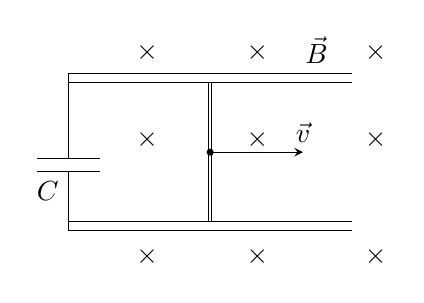
\begin{tikzpicture}[>=stealth]

\draw (0,.92)--(0,2)--(3.6,2) (0,.76)--(0,0)--(3.6,0) (-.4,.76)--(.4,.76) (-.4,.92)--(.4,.92);
\draw (0,1.88)--(3.6,1.88) (0,.12)--(3.6,.12);\draw[double] (1.8,.12)--(1.8,1.88);
\node[below left]at(0,.75){$C$};\draw[->] (1.8,1)--(2.98,1)node[above]{$\vec v$};\fill (1.8,1)circle(.045);
\foreach \x in {1,2.4,3.9}{\foreach \y in {-.32,1.16,2.26}{\node at(\x,\y){$\times$};}}
\node[above]at(3.15,2){$\vec B$};
\end{tikzpicture}\end{center}
По двум горизонтально расположенным параллельным проводящим рельсам с пренебрежимо малым сопротивлением, замкнутым на конденсатор электроёмкостью С  =  $100$ мкФ, поступательно и равномерно скользит проводящий стержень. Расстояние между рельсами l  =  $1\,\text{м}$. Рельсы со стержнем находятся в вертикальном однородном магнитном поле с индукцией B  =  $1$ Тл (см. рис.). Через достаточно большой промежуток времени от начала движения энергия электрического поля конденсатора W  =  $50$ мкДж. Какова скорость движения стержня? Рельсы закреплены на диэлектрической подложке.
}{
\smallskip\noindent\textbf{Решение}\par
$1$.  Модуль ЭДС индукции, возникающей в контуре при движении стержня: $|\mathcal E|=B v l,$где B  — модуль вектора магнитной индукции, \ensuremath{\upsilon}  — скорость движения стержня, l  — длина стержня. 
$2$.  Так как напряжение на конденсаторе $U_{c}$ равно модулю ЭДС индукции, то энергия электрического поля конденсатора определяется по формуле: 

\[W= \frac{C U_C ^2}{2} = \frac{C B ^2 v ^2 l ^2}{2} .\]

В итоге скорость стержня равна: 

\[v = \sqrt{\frac{2 W}{C B ^2 l ^2}} = \sqrt{\frac{2 \cdot 50 \cdot 10^{-6}}{100 \cdot 10 ^{ - 6 } \cdot 1 ^2 \cdot 1 ^2}} =1 \,\text{м} / \,\text{с}.\]

Ответ: $1\,\text{м/с}$.
}

% Source 4756: https://phys-ege.sdamgia.ru/problem?id=4756
\BankTask{4756}{
\begin{center}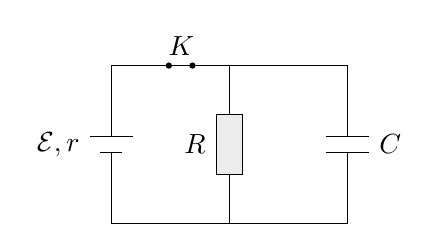
\begin{tikzpicture}[>=stealth]

\draw(0,0)--(3,0)--(3,.9) (3,1.1)--(3,2)--(1.03,2) (.73,2)--(0,2)--(0,1.1) (0,.9)--(0,0);
\draw(.73,2)--(1.03,2);\fill(.73,2)circle(.04) (1.03,2)circle(.04);\node[above]at(.89,2){$K$};
\draw(-.27,1.1)--(.27,1.1) (-.14,.9)--(.14,.9) (2.73,1.1)--(3.27,1.1) (2.73,.9)--(3.27,.9);
\draw(1.5,0)--(1.5,.62) (1.5,1.38)--(1.5,2);\draw[fill=gray!15](1.33,.62)rectangle(1.67,1.38);
\node[left]at(-.28,1){$\mathcal E,r$};\node[left]at(1.32,1){$R$};\node[right]at(3.28,1){$C$};
\end{tikzpicture}\end{center}
В электрической схеме, показанной на рисунке, ключ К замкнут. ЭДС батарейки $\mathcal E = 12\,\text{В},$ емкость конденсатора $C = 0{,}2\,\text{мкФ}.$ Отношение внутреннего сопротивления батарейки к сопротивлению резистора $k= \frac{r}{R} =0{,}2.$ Найдите количество теплоты, которое выделится на резисторе после размыкания ключа К в результате разряда конденсатора.
}{
\smallskip\noindent\textbf{Решение}\par
Когда ключ замкнут, конденсатор заряжен, а через резистор течет ток, который можно найти, применив закон Ома для полной цепи:

\[I= \frac{\mathcal E}{R + r} .\]

Поскольку резистор и конденсатор подключены параллельно, напряжения на них совпадают и равны:

\[U = IR = \frac{R \mathcal E}{R + r} .\]

После размыкания ключа, конденсатор разряжается через сопротивление, и вся накопленная в нем энергия электрического поля переходит в тепло. Таким образом, искомое количество теплоты равно:

\[Q= \frac{CU ^2}{2} = \frac{C}{2} ( \frac{\mathcal E}{1 + r/R} ) ^2 = \frac{0{,}2 \cdot 10 ^{ - 6 } \,\text{Ф}}{2} \cdot ( \frac{12\,\text{В}}{1 + 0{,}2} ) ^2 = 10 ^{ - 5 } \,\text{Дж}.\]

Ответ: $10 ^{ - 5 } \,\text{Дж}.$
}

% Source 32269: https://phys-ege.sdamgia.ru/problem?id=32269
\BankTask{32269}{
\begin{center}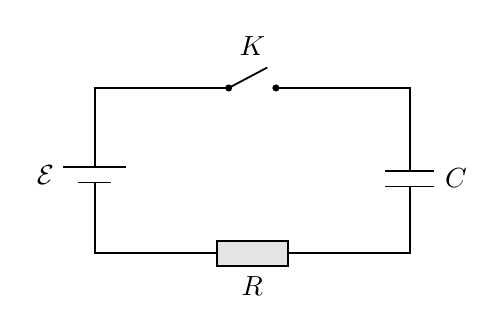
\begin{tikzpicture}[>=stealth,line width=.65pt]\draw (0,1.1)--(0,2.1)--(1.7,2.1) (2.3,2.1)--(4,2.1)--(4,1.05) (4,.85)--(4,0)--(2.45,0) (1.55,0)--(0,0)--(0,.9);\draw (-.4,1.1)--(.4,1.1) (-.21,.9)--(.21,.9) (3.69,1.05)--(4.31,1.05) (3.69,.85)--(4.31,.85);\draw (1.7,2.1)--(2.19,2.36);\foreach \x in {1.7,2.3}{\fill (\x,2.1) circle (.045);}\draw[fill=gray!20](1.55,-.16)rectangle(2.45,.16);\node[left]at(-.39,1){$\mathcal E$};\node[right]at(4.32,.95){$C$};\node[below]at(2,-.17){$R$};\node[above]at(2,2.38){$K$};\end{tikzpicture}\end{center}

Незаряженный конденсатор с емкостью C  =  $0{,}1$ мкФ подключают к источнику тока по схеме, показанной на рисунке. Сопротивление резистора R  =  $500\,\text{Ом}$, сопротивлением проводов и внутренним сопротивлением источника можно пренебречь. После замыкания ключа К на резисторе выделяется тепло равное $7{,}2$ мкДж. Чему равно ЭДС источника?
}{
\smallskip\noindent\textbf{Решение}\par
При замыкании цепи через резистор проходит ток зарядки до тех, пока конденсатор не зарядится до напряжения, равного ЭДС источника тока.
При этом через источник тока протечет заряд, равный $q=CU=C \mathcal{E} .$ Тогда в источнике тока будет совершена работа $A=q \mathcal{E} =C \mathcal{E} ^2 .$
Энергия, которую приобретет при этом заряженный конденсатор, равна:

\[W_{\,\text{р}}= \frac{CU ^2}{2} = \frac{C \mathcal{E} ^2}{2} .\]

Поскольку сопротивлением проводов и внутренним сопротивлением источника тока можно пренебречь, то можно применить закон сохранения энергии:

$A_{\,\text{ист}}=Q + W_p,$
$C \mathcal{E} ^2 =Q + \frac{C \mathcal{E} ^2}{2} ,$

 откуда:

\[\mathcal E=\sqrt{\frac{2Q}{C}}=\sqrt{\frac{2\cdot7{,}2\cdot10^{-6}}{0{,}1\cdot10^{-6}}}=12\,\text{В}.\]

Ответ: $12\,\text{В}$.
}

\end{document}
